%        File: sheet.tex
%     Created: Mon Mar 14 04:00 PM 2016 C
% Last Change: Mon Mar 14 04:00 PM 2016 C
%
\documentclass[a4paper,twocolumn]{article}

\usepackage{geometry}
\usepackage{amsmath}
\usepackage{graphicx}
\usepackage{float}

\geometry{a4paper, margin={.3in, .3in}}

\title{Computer Vision 1 \\ Cheat Sheet}
\author{Andrea Jemmett}

\begin{document}
\maketitle

\section{Color Models}
Color is part of the electromagnetic spectrum with energy in the range from 380
to 780 nm wavelength. Most of the colors we perceive are a mixture of
wavelengths where the amount of energy at each wavelength is given by the
spectral energy distribution (SED). When white light shines upon an object, some
wavelengths are absorbed and other are reflected (a green object will reflect
light with wavelength around 500nm, other wavelengths will be absorbed). The
\textbf{hue} corresponds with the dominant wavelength of the SED;
\textbf{saturation} is defined as the proportion of pure light with respect to
white light needed to produce the color; \textbf{lightness} is the intensity of
the reflected light meanwhile \textbf{brightness} is the intensity of the light
source. Let $EH$ be the dominant wavelength in the SED and $EW$ the wavelength
contributing to the white light, then the \textit{hue} is equal to $EH$, the
\textit{saturation} equals to the difference $EH - EW$ and the
\textit{lightness} equals to the area underlined by the SED.

\begin{figure}[htpb]
	\centering
	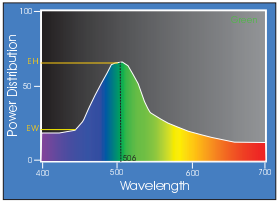
\includegraphics[height=1.5in]{imgs/color-sed.png}
\end{figure}

Experiments have been conducted in which a human observer was asked to adjust
three knobs which control the intensity of a three primary colors so to match
the (perceived) color of the test light. The three primary lights were
additively mixed in and the knobs' values were recorded yielding the so called
color matching functions $\bar{r}(\lambda)$, $\bar{g}(\lambda)$ and
$\bar{b}(\lambda)$. The problem with these was that a negative amount of
at least one of the primaries was necessary to produce the full spectra. So the
CIE proposed a mathematical transformation, the \textbf{XYZ} model, which uses
another set of color matching functions: $\bar{x}(\lambda)$, $\bar{y}(\lambda)$
and $\bar{z}(\lambda)$.

The observer perceives color in terms of three color signals based on the
trichromacy theory and can be modeled as:

\begin{equation} \label{eq:color-perception}
C = \int_{\lambda} E(\lambda) S(\lambda) f_C(\lambda) d\lambda
\end{equation}

where $C \in \{R, G, B\}$, $E$ is the SPD, $S$ is the light reflected by objects
and $f_C$ is the color matching function. If we use $\bar{x}$, $\bar{y}$ and
$\bar{z}$ then we have the XYZ color space. To better represent graphically this
color space we can compute the $xyz$ values as follows:

\begin{equation}
x = \frac{X}{X + Y + Z} \quad y = \frac{Y}{X + Y + Z} \quad z = \frac{Z}{X + Y + Z}
\end{equation}

where we factor out the intensity. Since the chromaticity values sum to unity,
two elements are sufficient to represent a color. When the $x$ and $y$ values
are represented on a plane the chromaticity diagram is obtained. We can also
infer the hue from the chromaticity diagram: first we need to select a reference
white light, the hue is then the wavelength at the spectral curve that
intersects the line from reference light through the color point to the spectral
curve (this point is $G_2$). If $||G_1||$ is the distance from the color to the
white light and $||G_2||$ is the distance from $G_2$ to the white source, then
the saturation is given by $\frac{||G_1||}{||G_2||}$.

RGB values can be obtained using equation \ref{eq:color-perception} and the
$\bar{r}$, $\bar{g}$, and $\bar{b}$ color matching functions. The projection of
RGB points on the rgb chromaticity triangle is defined by:

\begin{equation}
r = \frac{R}{R + G + B} \quad g = \frac{G}{R + G + B} \quad b = \frac{B}{R + G + B}
\end{equation}

In the HSI chromaticity diagram, we compute hue and saturation in the following
way: by assuming white light we define a reference point of $r = g = b = 1/3$,
the saturation can than be computed as:

\begin{equation}
S_{rgb}(r, g, b) = \sqrt{(r - 1/3)^2 + (g - 1/3)^2 + (b - 1/3)^2}
\end{equation}

or

\begin{equation}
S(R, G, B) = 1 - \frac{min(R, G, B)}{R + G + B}
\end{equation}

while the hue is given by:

\begin{equation}
H_{rgb}(r, g, b) = arctan(\frac{r - 1/3}{g - 1/3})
\end{equation}

or

\begin{equation}
H(R, G, B) = arctan(\frac{\sqrt{3}(G - B)}{(R - G) + (R - B)})
\end{equation}

A color invariant system contains color invariant models that are more or less
insensitive to the varying image conditions. For matte surfaces
\textit{RGB} is sensitive to orientation while \textit{rgb} is (assuming
constant white light) insensitive to orientation, illumination direction and
intensity (similarly are S and H). For shiny surfaces H is color invariant.


\section{Surface Reflection}



\section{Image Processing}


\end{document}

